\documentclass[submit]{ipsj}
%\documentclass{ipsj}

\usepackage[expert]{otf}
\usepackage[noalphabet]{pxchfon}
\setminchofont[0]{A-OTF-RyuminPr6-Light.otf}
\setgothicfont[0]{A-OTF-FutoGoB101Pr6-Bold.otf}

\usepackage[dvipdfmx]{graphicx}
\usepackage{latexsym}

\def\Underline{\setbox0\hbox\bgroup\let\\\endUnderline}
\def\endUnderline{\vphantom{y}\egroup\smash{\underline{\box0}}\\}
\def\|{\verb|}

\setcounter{巻数}{57}
\setcounter{号数}{1}
\setcounter{page}{1}


\受付{2015}{3}{4}
%\再受付{2015}{7}{16}   %省略可能
%\再再受付{2015}{7}{20} %省略可能
\採録{2015}{8}{1}

\usepackage[framemethod=TikZ]{mdframed}
\usepackage{amsmath, amssymb, amsthm}
\usepackage{minted}
\usemintedstyle{bw}
\usepackage{url}
\usepackage{ucolor}

\begin{document}


\title{定理証明支援系Coqにおける不等式変形記法}

\etitle{A Tactic Library for Transforming Inequalities in Coq}

\affiliate{KIT}{九州工業大学\\
Kyushu Institute of Technology}

\author{村田 康佑}{Kosuke Murata}{KIT}[murata@pl.ai.kyutech.ac.jp]
\author{江本 健斗}{Kento Emoto}{KIT}[emoto@ai.kyutech.ac.jp]

\begin{abstract}
数学定理やプログラムの性質の形式的証明では,自然数上の不等式についての証明が頻出する.しかし,定理証明支援系Coqでの不等式の形式的証明は,非形式的証明とは異なる記法で記述されるため,数学的な直観がそのまま使えないことも多い.例えば,非形式的証明では,不等式$L \leq R$を証明するために,しばしば$L = M_1 \leq M_2 = M_3 \leq \cdots \leq M_n = R$のように項を不等号で「鎖状」につなげて示す宣言的な記法が用いられる.こうした記法は数学の教科書などでよく馴染んだ記法であり,直観的に理解・記述することが可能である.一方,Coqにはそうした宣言的な記法は標準では用意されていないため,証明の理解・記述が困難になっている.本論文では,Coq上で,自然数上の不等式変形を,非形式的証明のように「鎖状」に記述する手法を提案する.本手法の特徴は,タクティックライブラリによって「鎖状」記法が実現されることにあり,それゆえ,提案記法はライブラリをモジュールとして読み込むだけで既存記法と併せて使うことができる.また,このタクティックライブラリを用いて,Ackermann関数の性質についての不等式の証明を試みる.その結果,標準的な数学の教科書と近い記法で形式的証明を記述できることを確認する.
\end{abstract}


\begin{jkeyword}
定理証明支援系,Coq,宣言的証明,タクティックライブラリ,不等式
\end{jkeyword}


% formal を動詞で使って形式化の意味になるのか?
\begin{eabstract}
Formal proofs of inequalities on natural numbers is important for formal proofs of mathematical theorems and properties of programs. However,  Coq's notation of formal proofs of inequalities is different from that of informal proofs. For instance, when we write an informal proof of inequality $L \leq R$, we usually use a declarative notation like a ``chain'' such that $L = M_1 \leq M_2 = M_3 \leq \cdots \leq M_n = R$. Such notation is common in textbooks, and thus it enables us to understand proofs intuitively. On the other hand, standard Coq does not support such a declarative notation, so that we cannot understand proofs in Coq intuitively. In this paper, we propose a novel approach to enable us to write formal proofs in the ``chain'' notation. One of main features of our approach is that the chain notation is realized as a tactic library, so that we can use it easily by only loading it as a module, and in conjunction with the conventional notation. We also try writing formal proofs for properties of Ackermann function with our tactic library. The result shows that we can write the formal proofs like informal proofs in a textbook.
\end{eabstract}

\begin{ekeyword}
proof assistant, Coq, declarative proof, tactic library, inequality
\end{ekeyword}

\maketitle

%1
\section{はじめに}

プログラム検証や数学の定理証明検証といった文脈で,Coq~\cite{09thecoq}やIsabelle/HOL~\cite{Nipkow:2002:IPA:1791547}などの定理証明支援系が有名である.これらのツールは,ユーザーが形式的証明を記述するのを補助し,また型検査器によって証明を検証するものである.典型的な成果としては,四色定理の証明の検証\cite{FourColorTheorem}やCコンパイラ~\cite{CompCert}の検証が有名である.また最近,Coqおよびその拡張であるSSReflect/MathComp についての日本語の教科書~\cite{hagiwara_afelt2018}が出版されるなど,国内でも注目されている.

しかし,定理証明支援系Coqでの形式的証明は,鉛筆(あるいはボールペン,万年筆,$\ldots$)でノート上に行う非形式的証明とは異なる記法や構造で記述されるため,数学的な直観がそのまま使えないことも多く,不便である.

本論文が目指す究極の目的は,証明を書く・証明を読むという2つの場面において,非形式と形式の間にある大きな溝を埋めることにある.より具体的な目標は,以下の2点について,Coqにおける形式的証明と非形式的証明の溝を埋めることである.
\begin{itemize}
\item \emph{記述性}:鉛筆等で紙上に証明を書くのと同じ感覚で,Coqによる形式的証明が作れるようになることを目指す.
\item \emph{可読性}:非形式的証明がそうであるように,完成したCoqスクリプトがCoqと対話することなく読めるようになることを目指す
\end{itemize}
もとより,全ての証明において非形的証明とCoqの形式的証明の差を埋めることは難しい.非形式的証明には,分野ごとに特有の記法や常識があるからである.それゆえ,まずはある特定の分野に絞って,非形式的証明と形式的証明の差異について整理することが必要になってくる.

本論文が対象とするのは,自然数上の不等式である.数学定理やプログラムの性質の形式的証明では,自然数上の不等式についての証明が頻出する.また,自然数や不等式は数学においてごく基本的な対象であるから,主定理が自然数上の不等式ではなかったとしても,その主定理を示すための補題として自然数上の不等式が現れることもある.身近な例としては,計算量の評価といった文脈で不等式上の自然数が重要になることがある~\cite{Cormen:2009:IAT:1614191}.それゆえ,自然数上の不等式について考察することは有用である.

% 自然数上の不等式など,大部分は証明が容易に自動化できるのではないかと思われるかもしれない.実際,簡単な自然数上の不等式は,\verb+omega+タクティックを使って自動的に証明することができる.しかし,実用的に現れる範囲の不等式であっても,証明の自動化には限度がある.例えば\verb+omega+タクティックは,Quantifier-freeなPresburger算術の論理式しか証明することができない.Presburger算術とは,自然数についての理論の一つであり,乗算$\times$についての公理を持たず,後者関数および加法についての公理のみをもつものである.それゆえ,\verb+omega+タクティックでは,乗算を含むような不等式の自動証明を行うことはできない\footnote{ただし,変数と定数を掛け合わせた形であったり,乗算が現れる部分項ををまとめて一つの変数に置き換えると乗算記号が除去できるような場合は,omegaタクティックでも証明できることがある.}.実は,乗算を含むような不等式の自動証明は,計算可能性の観点から本質的な難しさを伴っている.というのも,Hilbertの第10問題 \footnote{Hilbertの第10問題とは,今風の言葉で言えば,「$n$個の未知数を含む整数係数$f(x_1,\ldots,x_n) = 0$に対して,整数上の不定方程式$f(x_1,\ldots,x_n) = 0$が解を持つか否かを判定するアルゴリズムはあるか」という問題である.} が決定不能であることから,乗算を含む自然数上の不等式をすべて自動的に証明することは諦めざるを得ないことが言えるためである.

では,自然数上の不等式の証明において,非形式的証明とCoqによる形式的証明はどういった違いを孕んでいるだろうか.例題を通して考察する.ここでは,不等式
\begin{eqnarray}
\forall n : \mathbf{nat} \mathrel{,} 5 \leq n \to 2^{n + 1} \leq n! \label{fml:ineq}
\end{eqnarray}
の証明を考える.この不等式の証明は様々な方法がありうるが,非形式的な証明では\figref{fig:ineq_sample_informal}のような証明,Coqでの形式的証明では\figref{fig:ineq_sample_normal_notation}のスクリプトによる証明が,それぞれ典型的な例だと考えられる.ただし,\figref{fig:ineq_sample_normal_notation}のスクリプトに現れる \verb+n!+ は,\verb+Notation+コマンドを使って定義したものである.

\begin{figure}[t]
\begin{mdframed}
\begin{proof}
$n$についての帰納法による.
\begin{enumerate}
\item[(Base case)~] $n = 5$のとき,
\begin{eqnarray*}
\begin{array}{ll}
&\text{(左辺)}\\
=& 2^{5 + 1} \\
=& 64 \\
\leq& 120 \\
=& 5!\\
=&\text{(右辺)}.
\end{array}
\end{eqnarray*}
\item[(Induction step)~] $n$の場合を仮定する.すると,$n + 1$の場合も
\begin{eqnarray*}
\begin{array}{lll}
&\text{(左辺)}\\
=& 2^{(n + 1) + 1} \\
=& 2 \cdot 2^{n + 1} \\
\leq& 2 \cdot n! & \text{\small (帰納法の仮定より)}\\
\leq& (n + 1) \cdot n! & \text{\small ($2 \leq n + 1$より)}\\
=& (n + 1)! \\
=&\text{(右辺)}
\end{array}
\end{eqnarray*}
より成り立つ.\qedhere
\end{enumerate}
\end{proof}
\end{mdframed}
\caption{不等式$\forall n : \mathbf{nat} \mathrel{,} 5 \leq n \to 2^{n + 1} \leq n!$の典型的な非形式的証明}
\ecaption{A typical informal proof for inequality $\forall n : \mathbf{nat} \mathrel{,} 5 \leq n \to 2^{n + 1} \leq n!$.}
\label{fig:ineq_sample_informal}
\end{figure}

\begin{figure}[t]
\begin{mdframed}
\begin{minted}[xleftmargin=10pt, linenos, numbersep=8pt]{coq}
Lemma sampl_ineq_prop :
    forall (n : nat), 5 <= n -> 2^(n+1) <= n!.
Proof.
  intros n H.
  induction H.
  - simpl; omega.
  - simpl.
    apply Nat.add_le_mono; auto.
    rewrite Nat.add_0_r.
    rewrite <- Nat.mul_1_l at 1.
    apply Nat.mul_le_mono; auto.
    omega.
Qed. 
\end{minted}
\end{mdframed}
\caption{不等式$\forall n : \mathbf{nat} \mathrel{,} 5 \leq n \to 2^{n + 1} \leq n!$を証明する典型的なCoqスクリプト}
\ecaption{A typical Coq script for proving a inequality $\forall n : \mathbf{nat} \mathrel{,} 5 \leq n \to 2^{n + 1} \leq n!$.}
\label{fig:ineq_sample_normal_notation}
\end{figure}
\figref{fig:ineq_sample_informal}と\figref{fig:ineq_sample_normal_notation}を見比べてみると,Coqスクリプトによる形式的証明は,非形式的証明に対して以下のような短所をもっていることに気づく.
\begin{itemize}
\item 形式的証明は,非形式的証明に比してより多くの変数が現れており,しかもそれぞれの変数がどういう型を持っているのかがスクリプト上からはわからない.このことを定理証明という文脈で言い直せば,証明中に仮定の名前がたくさん現れるが,それぞれの仮定が具体的に何かはわからないということになる.例えば,\figref{fig:ineq_sample_normal_notation}の形式的証明では\verb+n+の他にも,\verb+H+といった変数(仮定)が現れているが,Coqとの対話なしで\verb+H+が何をさしているのか理解するのは難しい.これはスクリプトを証明として読む場合の可読性を大きく下げる原因となっている.
\item 非形式的証明では,「左辺を変形して右辺にする」という方針で証明がなされている.そのため,不等式$L \leq R$を証明するために,$L = M_1 \leq M_2 = M_3 \leq \cdots \leq M_n = R$のように項を等号や不等号で鎖状につなげて示す記法が用いられている(以下では,この記法を\emph{鎖状記法}という).ここでは,$M_1, \ldots , M_n$といった項に注目をして逐次的変形が進められることによって証明が完成している.一方,形式的証明では,ゴールの不等式全体に注目して,それを「自明な不等式に還元する」ことで証明を完成させている.例えば,\figref{fig:ineq_sample_normal_notation}のスクリプトの8行目に現れている\verb+apply+タクティックと\verb+auto+タクティックの連続は,\verb+Nat.add_le_mono+ ($\forall \; m \; m \; p \; q : \mathbf{nat} \mathrel{,} n \leq m \to p \leq q \to n + p \leq m + q$)を用いて,現在のサブゴール
\[
\varGamma \vdash 2^{m + 1} + (2^{m + 1} +0) \leq m! + m \cdot m!
\]
を,より簡単な不等式
\[
\varGamma \vdash 2^{m + 1} + 0 \leq m \cdot m!
\]
へと書き換えている.もとより,非形式的証明においてもこうした「自明な不等式に還元する」方法が使われないわけではなく,「左辺を変形して右辺にする」方法と併用されているというべきであろう.しかし,Coqの非形式的証明においては鎖状記法はそもそもサポートされていないため,2つの記法が併用できる非形式的証明に比して不自由な思考を強いてしまっていると言える.
\end{itemize}

以上,Coqにおける形式的証明の短所を2点指摘した.このうち前者については,適切にコメントやアノテーションを施すことによってある程度緩和することができる.例えば\verb+H+という変数が何を指しているかわからなければ,スクリプト上に\verb+H+が何を指しているのかメモしておけば良いということである.

一方,後者はより深刻な問題である.「左辺を変形して右辺にする」という証明の方針をサポートするためには,ぜひとも鎖状記法をサポートするべきである.

本論文では,不等式の鎖状記法をサポートするためのタクティックライブラリを設計し,タクティック記述言語Ltacを用いて実装した.このライブラリの使用例として,不等式(\ref{fml:ineq})の証明を記述したスクリプトを\figref{fig:ex_proof_ineq}に示す.このスクリプトを例にして,本論文で実装したタクティックライブラリの特徴について説明する.このスクリプトの証明では帰納法が用いられているが,base case と induction step のそれぞれについて,左辺から右辺へ至る項の変形の過程が明示的に書かれていることがわかる.特に,\figref{fig:ineq_sample_normal_notation}の非形式的証明と同様に,
\begin{itemize}
\item ステップごとの変形の結果と,
\item ステップごとの変形ができる理由 (ただし自明な場合は省略できる)
\end{itemize}
が明示的に表れている点に注目されたい.例えば,スクリプトの18行目から19行目は,\verb+IHle+を理由にして,\verb-(2 * (S m + 1)) <= (2 * m !)- なる不等式変形ができることを示している.また,アノテーションによって,現在のサブゴールや重要な変数の型がスクリプト中に明示的に現れていることにも注目されたい.例えば,スクリプトの8, 14, 15行目には,現在のサブゴールや変数\verb+IHle+の型の情報が明示的に書かれている.このアノテーションは単なるコメントではなく,Coqの型チェックを呼び出すタクティックとして設計されており,現在のコンテクストと整合しない記述は型チェックによって弾かれるようになっている.これらの機序によって,Coqを知らないユーザであっても,十分にこのスクリプトは理解できると考えられる.

\begin{figure}[t]
\begin{mdframed}
\begin{minted}[xleftmargin=10pt, linenos, numbersep=8pt]{coq}
Lemma sampl_ineq_prop :
  forall (n : nat), 5 <= n -> 2^(n+1) <= n!.
Proof.
  intros n H.
  @ H : (5 <= n).
  induction H.
  (* base case : n = 5 *)
  - @ goal : (2 ^ (5 + 1) <= 5!).
    Left
    = 64.
    <= 120   { omega }.
    = Right.
  (* induction step *)
  - @ goal : (2 ^ (S m + 1) <= (S m)!).
    @ IHle : (2 ^ (m + 1) <= m !).
    Left
    = (2 ^ (S m + 1)).
    = (2 * 2 ^ (m + 1)).
    <= (2 * m !)     { by IHle }.
    <= ((S m) * m !) 
               { because (2 <= (S m)) by omega }.
    = ((S m)!).
    = Right.
Qed.
\end{minted}
\end{mdframed}
\caption{提案するタクティックライブラリを用いて不等式$\forall n : \mathbf{nat} \mathrel{,} 5 \leq n \to 2^{n + 1} \leq n!$を証明するスクリプト}
\ecaption{A script for proving $\forall n : \mathbf{nat} \mathrel{,} 5 \leq n \to 2^{n + 1} \leq n!$ using novel tactic library}
\label{fig:ex_proof_ineq}
\end{figure}

また本論文では,提案する手法の評価として,実装したタクティックライブラリを用いて,Ackermann関数の諸性質の形式的証明を,非形式的な証明に似た可読性の高い記法で記述できることを示す.

なお,本論文を読む上で,以下の点に注意されたい.
\begin{itemize}
\item われわれは,本論文で提案する手法を Coq 8.7.0 で実装した.また,その実装が,少なくとも本論文で紹介した例の範囲では Coq 8.7.1でも正しく動作することを確かめた.
\item 本論文中にはいくつかCoqのスクリプトが現れるが,典型的なモジュールのインポートやnotationの定義は省略している.
\item 本論文で述べる手法の実装および,その実装の評価のために作成した証明は,Web上の以下のURLで公開している: \url{https://github.com/MurataKosuke/Inequality}
\end{itemize}

これ以降の本論文の構成は以下の通りである.2章では,関連研究の紹介と,本論文との比較を行う.3章では,タクティックライブラリの設計と実装の基本方針について述べる.4章では,3章で述べた方針を受けて,タクティックライブラリをさらに使いやすいものにするためのアイデアとその実装について述べる.5章では,本論文で提案するタクティックライブラリを用いた有意義な命題の例として,Ackermann関数の性質についての証明について述べる.最後に,6章で本論文のまとめと将来の課題について検討を行う.

%本論文で提案する記法は,自然数上の不等式の証明についてのものであるが,そうした不等式の大部分は証明が容易に自動化できるのではないかと思われるかもしれない.実際,簡単な自然数上の不等式は,\verb+omega+タクティックを使って自動的に証明することができる.

%しかし,実用的に現れる範囲の不等式であっても,証明の自動化には限度がある.例えば\verb+omega+タクティックは,Quantifier-freeなPresburger算術の論理式しか証明することができない.Presburger算術とは,自然数についての理論の一つであり,乗算$\times$についての公理を持たず,後者関数および加法についての公理のみをもつ.それゆえ,\verb+omega+タクティックでは,乗算を含むような不等式の自動証明を行うことはできない\footnote{ただし,変数と定数を掛け合わせた形であったり,乗算が現れる部分項ををまとめて一つの変数に置き換えると乗算記号が除去できるような場合は,omegaタクティックでも証明できることがある.}.実は,乗算を含むような不等式の自動証明は,計算可能性の観点から本質的な難しさを伴っている.というのも,Hilbertの第10問題 \footnote{Hilbertの第10問題とは,今風の言葉で言えば,「$n$個の未知数を含む整数係数$f(x_1,\ldots,x_n) = 0$に対して,整数上の不定方程式$f(x_1,\ldots,x_n) = 0$が解を持つか否かを判定するアルゴリズムはあるか」という問題である.} が決定不能であることから,乗算を含む自然数上の不等式をすべて自動的に証明することは諦めざるを得ないことが言えるためである.

\section{関連研究}

本章では,本論文の関連研究について述べる.我々の知る限りでは,不等式の証明や不等式変形の記述に特化したライブラリは先に例がない.しかし,等式変形や宣言的証明といった観点から探してみると,いくつか関連研究を見つけることができる.

\subsection{等式変形について}

等式変形の記述についての既存研究として,Tessonらのプログラム運算のためのタクティックライブラリ~\cite{10.1007/978-3-642-17796-5_10}があげられる.プログラム運算とは,プログラムの代数的性質を利用して意味を保存したままプログラムを変形し,高速なプログラムを得る技法であり,Bird-Meertens formalism (BMF) といわれる体系が有名である.Tessonらは,BMFに基づく等式運算を,Birdによるプログラム運算のレクチャーノート~\cite{Bird:1987:ITL:42675.42676}に出てくるような形で書くためのタクティックライブラリを与えている.プログラム運算という領域に特化したタクティックライブラリではあるが,等式変形を記述するための枠組みとして使用することもできる.しかし,本論文でサポートするような不等式変形までは具体的にはサポートしていない.

本論文は,Tessonらのアイデアが,等式変形のみならず自然数上の不等式変形にも部分的に適用可能であることを示したものであり,また自然数上の不等式変形で生じる特有の問題について考察を加えたものである.また,本論文で実装したタクティックライブラリは,Tessonらのタクティックライブラリの実装を参考にしつつ,そのアイデアを自然数上の不等式変形へと拡張したものである.

\subsection{宣言的証明について}

各ステップにおけるゴールを明示的に記述するような証明の記法を,宣言的記法という.定理証明支援系において宣言的記法を実現する試みはいくつかある.Isabelle/HOLをベースにした宣言的証明記述言語の設計としてIsar~\cite{Bauer:2001:CRR:646528.695193} が有名であるが,Coq でもCorbineauによる新たな証明記述言語の実装~\cite{10.1007/978-3-540-68103-8_5}がある.この研究は,全体にわたって自然言語に近い形で証明を記述できるように言語をデザインするものである.そのなかには,等式変形を鎖状に近い記法で記述するためのシンタクスもあり,その点では本論文と同じアプローチによる実装が含まれていると言える.

Corbineauによる手法~\cite{10.1007/978-3-540-68103-8_5}では,Coqをベースにしつつも新たな言語を設計しなおしていた.それゆえ,処理系を得るためには既存のCoq処理系を再コンパイルすることが必要になる.一方,われわれの手法では,新たな記法がLtacの範疇で実装したタクティックライブラリとして実現されており,既存のCoq処理系でタクティックライブラリを読み込むだけで使用できるという点に特徴を持つ.

\section{鎖状記法の設計と実装}

本章では,提案する手法の概要について述べる.

\subsection{タクティックライブラリの設計の概要}

本手法で提案するタクティックライブラリの設計について,概要を述べる.本手法は,あとで述べるように,少し注意すれば,
\begin{itemize}
\item 右辺から左辺に至る項の変形
\item 等号$=$および広義の不等号$\leq$のみならず狭義の不等号$<$の現れる不等式変形
\end{itemize}
へ拡張することができるが,まずは「左辺から右辺に至る,等号$=$および広義の不等号$\leq$が現れるような変形」を記述する手法に絞って解説する.

本論文で提案する手法の核心は,以下の4つの\verb+Tactic Notation+\footnote{Coqでは,\texttt{Tactic Notation}機能を用いると,タクティック記述言語Ltacを用いて,新たなタクティックとそのための記法を柔軟に設計することができる.}(以下,単にタクティックという)からなる.
\begin{itemize}
\item \underline{\gtfamily\bfseries タクティック1} ~\verb+Left = +$\langle\mathit{term}\rangle$\verb+ { +$\langle\mathit{tactic}\rangle$\verb+ }+
\item \underline{\gtfamily\bfseries タクティック2} ~\verb+= +$\langle\mathit{term}\rangle$\verb+ { +$\langle\mathit{tactic}\rangle$\verb+ }+
\item \underline{\gtfamily\bfseries タクティック3} ~\verb+<= +$\langle\mathit{term}\rangle$\verb+ { +$\langle\mathit{tactic}\rangle$\verb+ }+
\item \underline{\gtfamily\bfseries タクティック4} ~\verb+= Right+
\end{itemize}
これらのタクティックを用いて,$\Gamma \vdash t = s$や$\Gamma \vdash t \leq s$の形をしたサブゴールを示すことができる.具体的には,{\gtfamily\bfseries タクティック1}からはじめて,{\gtfamily\bfseries タクティック2},\,{\gtfamily\bfseries 3}を繰り返し用い,{\gtfamily\bfseries タクティック4}で証明を終える.これらのタクティックを並べると,あたかも項の変形の過程が鎖状に記されているかのように見えるのが重要な点である.\figref{fig:ex_proof_easy_prop}は,論理式$\forall \;x\;y\;z : \mathbf{nat}, \, x = y \to y \leq z \to x \leq z$を示すスクリプトであり,このスクリプトの 5 --- 9 行目では非形式的証明のような不等式変形が書かれているように見えるが,よくみると上の4つのタクティックを並べているだけであることがわかる.
\begin{figure}[t]
\begin{mdframed}
\begin{minted}[xleftmargin=10pt, linenos, numbersep=8pt]{coq}
Proposition example :
  forall x y z : nat, x = y -> y <= z -> x <= z.
Proof.
  intros x y z H0 H1.
  Left
  = x   { reflexivity }.
  = y   { exact H0 }.
  <= z  { exact H1 }.
  = Right.
Qed.
\end{minted}
\end{mdframed}
\caption{核心となるタクティックのみを用いた単純なスクリプトの例}
\ecaption{An example of simple script using important tactics}
\label{fig:ex_proof_easy_prop}
\end{figure}

これらのタクティックは,具体的には次のような動作をする.
\begin{itemize}
\item \underline{\gtfamily\bfseries タクティック1}~ \verb+Left = +$\langle\mathit{term}\rangle$\verb+ { +$\langle\mathit{tactic}\rangle$\verb+ }+\\ 現在のサブゴール$\varGamma \vdash x \leq y$を,$\varGamma \vdash \langle\mathit{term}\rangle \leq y$に書き換える.ただし,その書き換えを行うため,$x = \langle\mathit{term}\rangle$をタクティック$\langle\mathit{tactic}\rangle$を用いて示し,それを使って現在のサブゴールに現れる左辺の$x$を$\langle\mathit{term}\rangle$へとrewriteする.つまり,以下のスクリプトと同じである.
\begin{mdframed}[leftmargin=10pt, rightmargin=10pt, skipabove=5pt, skipbelow=15pt]
\verb+let Hre := fresh "H" in (+
\verb+  assert (+$x$\verb+ = +$\langle\mathit{term}\rangle$\verb+) as Hre by +$\langle\mathit{tactic}\rangle$\verb+;+\\
\verb+  rewrite Hre at 1; clear Hre).+
\end{mdframed}
なお,\verb+let Hre := fresh "H" in+の部分は,一時的におく仮定である$x = \langle\mathit{term}\rangle$にフレッシュな変数を割り当てるために必要な記述である.

\item \underline{\gtfamily\bfseries タクティック2}~ \verb+= +$\langle\mathit{term}\rangle$\verb+ { +$\langle\mathit{tactic}\rangle$\verb+ }+ \\ {\gtfamily\bfseries タクティック1}と同様である.

\item \underline{\gtfamily\bfseries タクティック3}~ \verb+<= +$\langle\mathit{term}\rangle$\verb+ { +$\langle\mathit{tactic}\rangle$\verb+ }+\\ 現在のサブゴール$\varGamma \vdash x \leq y$を$\varGamma \vdash \langle\mathit{term}\rangle \leq y$に書き換える.ただし,その書き換えを行うため,$x \leq \langle\mathit{term}\rangle$をタクティック$\langle\mathit{tactic}\rangle$を用いて示し,それと$\leq$の推移律から$\langle\mathit{term}\rangle \leq y$を導く.つまり,以下のスクリプトと同じである.
\begin{mdframed}[leftmargin=10pt, rightmargin=10pt, skipabove=5pt, skipbelow=15pt]
\verb+let Hre := fresh "H" in (+
\verb+  assert (+$x$\verb+ <= +$\langle\mathit{term}\rangle$\verb+) as Hre by +$\langle\mathit{tactic}\rangle$\verb+;+\\
\verb+  transitivity (+$\langle\mathit{term}\rangle$\verb+) ;+\\
\verb+  [ apply Hre | idtac ];+\\
\verb+  rewrite Hre; clear Hre).+
\end{mdframed}

\item \underline{\gtfamily\bfseries タクティック4}~ \verb+= Right+\\\verb+reflexivity+の言い換えである.
\end{itemize}

これらのタクティックは,いずれもLtacを用いて容易に実装することができる.というのも,Ltacには強力なパターンマッチの機能が用意されており,現在のサブゴールに現れる部分項を取得したり,その部分項を使って既存のタクティックを動かすことができるからである.

再び\figref{fig:ex_proof_easy_prop}のスクリプトを例にして,各タクティックの動きについて説明する.このスクリプトを,CoqIDE上でタクティックごとに読み込んだ様子が\figref{fig:interective}である.

\begin{figure}[t]
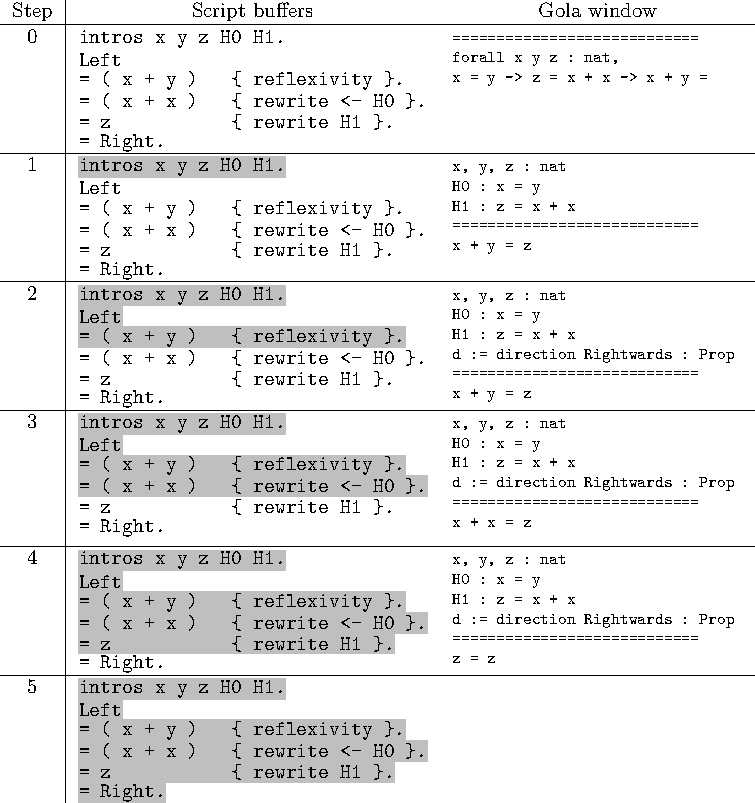
\includegraphics[width=\linewidth]{figure2.pdf}
\caption{CoqIDE上で\figref{fig:ex_proof_easy_prop}を読み込んだときの対話の様子}
\ecaption{Progress of interactive proof in Fig.\ref{fig:ex_proof_easy_prop} on CoqIDE}
\label{fig:interective}
\end{figure}

\begin{itemize}
\item Step 1は,Coq標準の\verb+intros+タクティックを用いているだけであるから問題ないだろう.
\item Step 2では,サブゴールは何も変化していないが,実際には\verb+assert (x = x) as H2 by reflexivity+によって\verb+H2 : x = x+なる項を型コンテキストに追加し,\verb+rewrite H2+で書き換えを行なったあと,\verb+clear H2+で\verb+H2+を削除している.
\item Step 3では,\verb+assert (x = y) as H2 by (exact H0)+によって\verb+H2 : x = y+なる項を型コンテキストに追加し,\verb+rewrite H2+で書き換えを行なったあと,\verb+clear H2+で\verb+H2+を削除している.
\item Step 4では,\verb+assert (y <= z) as H2 by (exact H1)+によって\verb+H2 : y <= z+なる項を型コンテキストに追加し,\verb+transitivity z+によって,2つのサブゴール``\verb+y <= z+''と``\verb+z <= z+''を得ている.前者は\verb+exact H0+によって証明を完了し,後者は\verb+idtac+により何もせずそのままにしておいている.それゆえ,Step4終了時のゴールとしては,\verb+z <= z+が残る.
\item 最後にStep5で,\verb+reflexivity+を呼び出して,証明を終了している.
\end{itemize}

なお,こうした素朴な実装では,{\gtfamily\bfseries タクティック1}よりも前に{\gtfamily\bfseries タクティック2}や{\gtfamily\bfseries タクティック3}が呼び出せてしまったり,式変形中に{\gtfamily\bfseries タクティック1}が複数回呼び出せてしまうという難点がある.もちろんそうしても正しい形式的証明は得られるが,鎖状記法による証明として人間が読むには意味のわからないものになってしまう.それゆえ,ぜひともこうした(スクリプトを人間が読む上では)意味のわからないタクティックの適用順を排除する機序が欲しい.実は,これは次節で述べる方法と同じ方法で実現できる.

\subsection{右辺から左辺に至る記法への対応}

前節では,左辺から右辺に至る方向(以下この変形の方向をrightwardsという)への変形を記述するタクティックについて説明した.これとほぼ同様の手法で,右辺から左辺に至る方向(以下この変形の方向をleftwardsという)への変形を記述するためのタクティックを実装することができる.具体的には,{\gtfamily\bfseries タクティック1},{\gtfamily\bfseries タクティック3},{\gtfamily\bfseries タクティック4}の代わりに以下の3つのタクティックを実装し,{\gtfamily\bfseries タクティック2}を左辺でなく右辺を書き換えるようにすればよい.
\begin{itemize}
\item \underline{\gtfamily\bfseries タクティック5}~  \verb+Right = +$\langle\mathit{term}\rangle$\verb+ { +$\langle\mathit{tactic}\rangle$\verb+ }+\\現在のサブゴールが$\varGamma \vdash x \leq y$のとき,$y = \langle\mathit{term}\rangle$を$\langle\mathit{tactic}\rangle$により示し,右辺$y$を$\langle\mathit{term}\rangle$へ書き換える.
\item \underline{\gtfamily\bfseries タクティック6}~ \verb+>= +$\langle\mathit{term}\rangle$\verb+ { +$\langle\mathit{tactic}\rangle$\verb+ }+\\現在のサブゴールが$\varGamma \vdash x \leq y$のとき,$y \leq \langle\mathit{term}\rangle$を$\langle\mathit{tactic}\rangle$により示し,$\leq$の推移律を用いて右辺$y$を$\langle\mathit{term}\rangle$へ書き換える.
\item \underline{\gtfamily\bfseries タクティック7}~ \verb+= Left+\\\verb+reflexivity+と同様.
\end{itemize}
ところが,問題となるのはrightwardsな変形とleftwardsな変形を同時にサポートしたい場合である.というのも,{\gtfamily\bfseries タクティック2}を呼び出した時点での現在の変形の方向が,leftwardsかrightwardsかどちらだったか覚えていないと,左辺と右辺のどちらを書き換えたら良いかわからなくなるからである.

タクティックを正しい順序で呼び出している限り,rightwardsな変形の最初は{\gtfamily\bfseries タクティック1}で始まるし,leftwardsな変形の最初は{\gtfamily\bfseries タクティック5}で始まる.それゆえ,{\gtfamily\bfseries タクティック1}および{\gtfamily\bfseries タクティック5}が呼び出された時点で,変形の向きがrightwardsかleftwardsかを表すダミー項を追加しておけば,書き換えの方向を覚えておくことができる.そのダミー項のための型として,2つのデータ型
\begin{mdframed}[leftmargin=10pt, rightmargin=10pt, skipabove=5pt, skipbelow=5pt]
\begin{verbatim}
Inductive state : Type :=
  Rightwards : state
| Leftwards : state.
\end{verbatim}  
\end{mdframed}
および
\begin{mdframed}[leftmargin=10pt, rightmargin=10pt, skipabove=5pt, skipbelow=5pt]
\begin{verbatim}
Inductive memo (cs : state) : Prop :=
  s : memo cs.
\end{verbatim}
\end{mdframed}
を定義しておく.その上で,{\gtfamily\bfseries タクティック1}が呼び出されたら,タクティック
\begin{mdframed}[leftmargin=10pt, rightmargin=10pt, skipabove=5pt, skipbelow=5pt]
\begin{verbatim}
pose ( memo Rightwards ).
\end{verbatim}
\end{mdframed}
を呼び出すようにすれば,型コンテクストに
\begin{mdframed}[leftmargin=10pt, rightmargin=10pt, skipabove=5pt, skipbelow=5pt]
\begin{verbatim}
P := memo Rightwards : Prop
\end{verbatim}
\end{mdframed}
という仮定が追加される.{\gtfamily\bfseries タクティック5}が呼び出された場合も同様に\verb+memo Leftwards+なる項を型コンテキストに追加する.そうしておけば,Ltacのゴールのパターンマッチを用いて,型コンテクストに\verb+memo Rightwards : Prop+があるか\verb+memo Leftwards : Prop+があるか調べることで現在の書き換えの向きがわかるわけである.それゆえ,{\gtfamily\bfseries タクティック2}を変形の向きに応じて書き換える向きを変えたり,{\gtfamily\bfseries タクティック3}と{\gtfamily\bfseries タクティック4}をrightwardsな書き換えの時にしか呼び出せないようにするといったことが可能になる.

%ところで,非形式的証明では,不等式$L \leq R$を示すために,
%\begin{eqnarray*}
%&L = M_1 \leq \cdots \leq M_n = T \\ 
%&R = M_1' \geq \cdots \geq M_m' = T
%\end{eqnarray*}
%のように,「左右から同じ項$T$へ合流する」ような変形をすることもある.これまでと同様に注意深くタクティックを作成することで,こうした記述をサポートすることも可能である.具体的には,まずデータ型 \verb~state~ に,中断を表す \verb~Temp~ を追加し,また同時に以下のタクティックを作れば良い.
%\begin{description}
%\item[タクティック8]\label{tactic5} \verb~= Temp~\\仮定に\verb+memo Rightwards : Prop+または\verb+memo Leftwards : Prop+なるダミー項あるとき,そのダミー項を一度削除し,新たなダミー項\verb+memo Temp : Prop+を追加し,さらに$l = $また,すでに仮定にダミー項\verb+memo Temp : Prop+があるときには,その
%\end{description}

\subsection{狭義の不等号}

これまで,広義の不等号(すなわち,$\leq$と$\geq$)における鎖状記法について議論した.しかし,ゴールが$L < R$のような狭義の不等号(すなわち,$<$と$>$)による不等式になっている場合について考えると,これまでのタクティックだけでは対応できない.

ひとまずrightwardsな変形のみを考える.狭義の不等号による不等式を鎖状記法により証明するために,以下の2点を拡張することが必要である.
\begin{enumerate}
\item {\gtfamily\bfseries タクティック2}を,$<$にも対応できるように拡張する.具体的には,{\gtfamily\bfseries タクティック2}について,さらに以下のルールを追加すればよい:現在のサブゴールが$\varGamma \vdash x < y$を$\varGamma \vdash \langle\mathit{term}\rangle < y$に書き換えるようにする.ただし,その書き換えを行うため,$x < \langle\mathit{term}\rangle$をタクティック$\langle\mathit{tactic}\rangle$を用いて示し,それと$<$の推移律から$\langle\mathit{term}\rangle < y$をゴールにする.
\item\label{item:point2} 新たなタクティック 
\begin{quote}
\quad\verb+< +$\langle\mathit{term}\rangle$\verb+ {+$\langle\mathit{tactic}\rangle$\verb+}+
\end{quote}
を実装する.このタクティックは,以下のような動作をする:現在のサブゴール$\varGamma \vdash x < y$を$\varGamma \vdash \langle\mathit{term}\rangle \leq y$に書き換えるようにする.ただし,その書き換えを行うため,$x < \langle\mathit{term}\rangle$をタクティック$\langle\mathit{tactic}\rangle$を用いて示し,それと,
\begin{eqnarray}
x < \langle\mathit{term}\rangle \to \langle\mathit{term}\rangle \leq y \to x < y \label{fml:trans_lt_le_lt}
\end{eqnarray}
が成り立つことから,$\langle\mathit{term}\rangle \leq y$をゴールにする.
\end{enumerate}
上の2点のうち2点目について,「現在のサブゴール$\varGamma \vdash x < y$を,($\varGamma \vdash \langle\mathit{term}\rangle < y$ではなく) $\varGamma \vdash \langle\mathit{term}\rangle \leq y$にする」という点が重要である.つまり,このタクティックが呼び出されたおかげで,ゴールに現れる不等号を$<$から$\leq$へと変えるわけである.というのも,広義の不等号は\verb~reflexivity~が成り立たないので,$<$のままでは{\bfseries\gtfamily タクティック4} (\verb+= Right.+)で証明を終わることができないからである.幸いにして,(\ref{fml:trans_lt_le_lt})式は常に成り立つので,いつでもこのような書き換えを行うことができる.


\subsection{自明なタクティックの省略}\label{subsec:easy_tactic}

\figref{fig:ex_proof_easy_prop}のスクリプトの5 --- 6行目において,\verb+x = x+を示すためのタクティックとして\verb+reflexivity+タクティックを指定しているが,この記述は冗長である.なぜならば,\verb+x = x+を示すために\verb+reflexivity+を用いるのは当たり前だからである.このように適用するタクティックが自明な場合には,\verb+{+$\mathit{tactic}$\verb+}+部を省略できるようにしたい.

そのためには,{\gtfamily\bfseries タクティック1}に加えて,新たに
\begin{itemize}
\item \underline{\gtfamily\bfseries タクティック1$'$}~ \label{tactic1'} \verb+Left = +$\langle\mathit{term}\rangle$
\end{itemize}
を実装すれば良い.この{\gtfamily\bfseries タクティック1$'$}は,ほとんど{\gtfamily\bfseries タクティック1}と同様だが,$x = \langle\mathit{term}\rangle$の証明を$\langle\mathit{tactic}\rangle$で行うのではなく,例えば
\begin{mdframed}[leftmargin=10pt, rightmargin=10pt, skipabove=10pt, skipbelow=10pt]
\begin{verbatim}
(simpl;reflexivity) || easy || auto
\end{verbatim}
\end{mdframed}
で行うようにすればよい.これは,\verb+simpl;reflexivity+,\verb+easy+,\verb+auto+を順番に試すものである.これで自明なタクティックは省略できるようになる.

また,{\gtfamily\bfseries タクティック1}~の$\langle\mathit{tactic}\rangle$の部分には,以下のパターンもよく現れる.
\begin{itemize}
\item \verb+rewrite +$H$
\item \verb+assert +$t$\verb+ as +$H$\verb+ by +$\langle\mathit{tactic}\rangle$\verb+;+\\
\verb+rewrite +$H$\verb+; clear +$H$
\end{itemize}
これらについても,{\gtfamily\bfseries タクティック1}の実装の$\langle\mathit{tactic}\rangle$部分を上記に置き換えた以下のようなタクティックを用意しておくと便利である.
\begin{itemize}
\item \underline{\gtfamily\bfseries タクティック1$''$}~ \verb+Left = +$ \langle\mathit{term}\rangle$\verb+{ by +$H$\verb+ }+
\item \underline{\gtfamily\bfseries タクティック1$'''$}~\\\quad  \verb+Left = +$ \langle\mathit{term}\rangle$\verb+{ because +$t$\verb+ by +$H$\verb+ }+
\end{itemize}

{\gtfamily\bfseries タクティック1}のみならず,{\gtfamily\bfseries タクティック2},{\gtfamily\bfseries タクティック3},{\gtfamily\bfseries タクティック6}についても,同様に$\langle\mathit{tactic}\rangle$部を省略したタクティックを作ることができる.


\subsection{強力な自動証明タクティックとの併用}

本論文で提案するライブラリは,強力な自動証明タクティックと併せて使用することによって,変形の1ステップを人間が理解しやすい程度に大きなものにできるため,よりわかりやすい証明を記述できるようになることが期待される.具体的には,以下のようなタクティックと併用すると良い.
\begin{description}
\item[omegaタクティック] \verb+omega+タクティックは,加法のみからなる(したがって乗法を含まない)自然数上の等式や不等式\footnote{より厳密には,Presburger算術の論理式として表せる範囲のものということになる.}を自動証明するためのタクティックである.
\item[ringタクティック] \verb+ring+タクティックは,環(ring)や半環(semiring)上の多項式の等式を自動的に証明するタクティックである.Coqでの自然数型\verb~nat~は半環であるため,自然数上の多項式についての等式は\verb+ring+タクティックを用いて自動的に証明できる.
\end{description}

\subsection{アノテーション}

1章で指摘したように,スクリプトの可読性を向上するために,現在のゴールや重要な変数の型などをスクリプト中に明示しておくためのアノテーションが導入されるべきである.そこで,以下の2つのアノテーションを用意した.
\begin{itemize}
\item \verb+@+ $H$ \verb+:+ $t$
\item \verb+@ goal+ \verb+:+ $t$
\end{itemize}
上は変数$H$の型が$t$であることを表し,下は現在のサブゴールが$t$であることを表す.このアノテーションもLtacによる\verb+tactic notation+として実装することができる.具体的には,\figref{fig:annotation}のようにすればよい.この実装では,パターンマッチによってアノテーションの記述が現在のコンテクストにあっているかどうかを検査し,あっていなければ適切なエラーメッセージを表示して失敗するようになっている.
\begin{figure}[t]
\begin{mdframed}
\begin{minted}[xleftmargin=10pt, linenos, numbersep=8pt, breaklines]{coq}
Tactic Notation (at level 2)
       "@" ident(H1) ":" constr(t) :=
  match goal with
  | [ H : t |- _ ] =>
    match H with
    | H1 => idtac "Type Annotation:" ; idtac "OK, "H":"t"is in current environment."
    | _  => fail 2 "Type Annotation Error: No such identifier"H1"that is typed"t
    end
  | _ => fail 2 "Type Annotation Error: No such identifiers that is typed"t
  end.

Tactic Notation (at level 2)
       "@" "goal" ":" constr(t) :=
  match goal with
  | [ |- t ] => idtac "OK, current goal is"t
  | [ |- ?t1 ] => fail 2 "Current goal is not"t", but is"t1
  end.
\end{minted}
\end{mdframed}
\caption{アノテーションの実装}
\ecaption{Implementation of annotations}
\label{fig:annotation}
\end{figure}

\section{Generalized Rewritingの利用}

本章では,Generalized Rewriting~\cite{JFR1574}を用いると,鎖状記法を用いた証明記述がより直観的になる場合があることを説明する.

\subsection{問題提起}\label{subsec:question}

突然だが,\figref{fig:need_generalized_rewriting}のスクリプトは,
\[
\begin{array}{l}
\forall x \; y : \mathbf{nat} \mathrel{,}\\
 x \leq y \to S\;(S\;(S\; (x^2))) \leq S\;(S\;(S\; (y^2)))
\end{array}
\]
の証明である.しかし,12行目の\verb+(* ??? *)+の部分が欠けていて不完全である.この部分には,$H : x \leq y$を仮定として
\begin{eqnarray}
S\;(S\;(S\; (x^2))) \leq S\;(S\;(S\; (y^2))) \label{fml:goal}
\end{eqnarray}
を示すタクティックを記述することになるが,何を記述するのが良いだろうか? もちろん,乗算を含む不等式なので\verb+omega+タクティックは使うことができない.
\begin{figure}[t]
\begin{mdframed}
\begin{minted}[xleftmargin=10pt, linenos, numbersep=8pt]{coq}
Proposition example :
  forall (x y : nat) ,
    x <= y ->
    S (S (S (x^2))) <= S (S (S (y^2))).
Proof.
  intros x y H.
  @ goal :
    (S (S (S (x^2))) <= S (S (S (y^2)))).
  @ H : (x <= y).
  Left
  =  (S (S (S (x^2)))).
  <= (S (S (S (y^2)))) { (* ??? *) }.
  = Right.
Qed.
\end{minted}
\end{mdframed}
\caption{例題: $\forall x \; y : \mathbf{nat} \mathrel{,} x \leq y \to S\;(S\;(S\; (x^2))) \leq S\;(S\;(S\; (y^2)))$を証明するスクリプト(ただし一部欠けていて不完全である)}
\ecaption{Example: a script of proving $\forall x \; y : \mathbf{nat} \mathrel{,} x \leq y \to S\;(S\;(S\; (x^2))) \leq S\;(S\;(S\; (y^2)))$ (Note that it is incomplete script, because of including a blank)}
\label{fig:need_generalized_rewriting}
\end{figure}

通常,(\ref{fml:goal})式のような不等式を示すとき,多くのCoqユーザーは,
\begin{itemize}
\item $\forall x\;y : \mathbf{nat}, \, x \leq y \to S\;x \leq S\;y$
\item $\forall x\;y : \mathbf{nat}, \, x \leq y \to x^2 \leq y^2$
\end{itemize}
のような命題の\verb+apply+を繰り返して,仮定$H : x \leq y$へと帰結させるのではないだろうか.この方針で証明を書くとすれば,仮に上の2つの命題を\verb+S_monotone+と\verb+sq_monotone+として,\verb+(* ??? *)+の部分に以下のようなタクティックを書くことになる.
\begin{mdframed}[leftmargin=10pt, rightmargin=10pt, skipabove=10pt, skipbelow=10pt]
\begin{verbatim}
repeat apply S_monotone; apply sq_monotone
; exact H
\end{verbatim}
\end{mdframed}
しかし,これはまさに(\ref{fml:goal})式の証明を構築するスクリプトそのものであり,もとの鎖状記法の中にこのスクリプトを書くのは不自然である.

直観的には,2乗$(-)^2$も後者関数$S$も$\leq$に関して単調であるのだから,そのまま$x$を$y$に書き換えたい.実は,そうした直観的な証明をCoq上で書く方法がある.端的にはgeneralized rewritingを用いれば良いのだが,次節以降でそれを詳しく説明する.

\subsection{Generalized Rewriting}

Coqの\verb+rewrite+タクティックは,Coqのデフォルトの等号  \verb+=+ がLeibniz equalityであることを利用して,\verb+t = s+であるときゴールに現れる\verb+t+を\verb+s+に書き換えるものである.実はこの\verb+rewrite+タクティックは,Coq標準ライブラリにある\verb+Setoid+モジュールを読み込むことで,等号のみならず様々な二項関係へ一般化して使うことができる.様々な二項関係といっても,同値関係へと一般化して使用するのが普通であるが,実際には推移的な関係であれば同値関係である必要はないし,本論文でも$\leq$といった同値関係でない関係に拡張する.

Generalized Rewritingのアイデアについて,本論文に関係する範囲で簡単に説明する.そのために,まずいくつか用語の定義をする.$A,B$を型とする.$A$上の2項関係$R$および$m : A$に対して,$m$が$R$のmorphismあるいはproper elementであるとは,$R\;m\;m$が成り立つことである.また,$A$上の2項関係$R$および$B$上の2項関係$R'$に対して,$A \to B$上の2項関係$R \mathrel{{+}\!\!{+}\!\!{\to}} R'$を以下のように定義する:
\begin{eqnarray*}
\lambda \;(f\;g : A \to B) , \; \forall \; (x \; y : A) , \; R\;x\;y \to R'\; (f\;x)\;(g\;y).
\end{eqnarray*}
特に,関数$f : A \to B$が,$A \to B$上の2項関係$R \mathrel{{+}\!\!{+}\!\!{\to}} R'$のmorphismであるとき,
\begin{eqnarray*}
\forall \; x \; y , \; R\;x\;y \to R'\; (f\;x)\;(f\;y)
\end{eqnarray*}
が成り立つことに注意されたい.例えば,後者$S$は${\leq} \mathrel{{+}\!\!{+}\!\!{\to}} {\leq}$のmorphismである.なぜならば,
\begin{eqnarray*}
\forall \; (x \; y : \mathbf{nat}) , \;x \leq y \to S\;x \leq S\;y
\end{eqnarray*}
が成り立つからである.

$A$を型とし,$R$を推移的な二項関係とする.ひとたび関数$f : A \to A$が$R \mathrel{{+}\!\!{+}\!\!{\to}} R$のmorphismだと示されると,以下の2つの推論ができるようになる:
\[
\frac{\varGamma,\, R\;x\;y \vdash  R\;(f\;y)\;t}{\varGamma,\,  R\;x\;y \vdash  R\;(f\;x)\;t} \qquad \frac{\varGamma,\, R\;x\;y \vdash  R\;t\;(f\;x)}{\varGamma,\,  R\;x\;y \vdash  R\;t\;(f\;y)}
\]
この推論が妥当であることは容易に示せる.重要な点は,上の2つの推論について,左の推論は$R\;x\;y$を理由にして$R\;(f\;y)\;t$を$R\;(f\;x)\;t$に書き換えることができると言っていると読めるし,右の推論は$R\;x\;y$を理由にして$R\;t\;(f\;x)$を$R\;t\;(f\;y)$に書き換えることができると言っていると読めるという点である.これが Generalized Rewriting のアイデアである.

上の規則について,わかりやすい例を挙げておく.$\leq$は推移的な二項関係であるし,後者$S$は${\leq} \mathrel{{+}\!\!{+}\!\!{\to}} {\leq}$のmorphismであったから,
\begin{eqnarray}
\frac{\varGamma,\,x \leq y \vdash  S\;y \leq t}{\varGamma,\,  x \leq y \vdash  S\;x \leq t} \qquad \frac{\varGamma,\, x \leq y \vdash  t \leq S\;x}{\varGamma,\, x \leq y \vdash  t \leq S\;y} \label{fml:twoset}
\end{eqnarray}
なる書き換えが可能である.この書き換えの妥当性は直観的に明らかだろう.


\subsection{CoqにおけるGneralized Rewriting}

Coqでは,標準ライブラリの\verb+Coq.Classes.Morphisms+上に,morphism (proper element) と$\mathrel{{+}\!\!{+}\!\!{\to}}$に対応する概念として,それぞれ\verb+Proper+型クラスと,\verb~++>~ 演算子が定義されている.それゆえ,例えば,後者$S$が${\leq} \mathrel{{+}\!\!{+}\!\!{\to}} {\leq}$のmorphismであることを,\verb~Proper (le ++> le) S~のインスタンスをつくる形で宣言することができる\footnote{$\leq$は,Coq上では関係\texttt{le}として定義されている.}.具体的には,以下のスクリプトのようにして宣言できる.
\begin{mdframed}[leftmargin=10pt, rightmargin=10pt, skipabove=5pt, skipbelow=5pt]
\begin{verbatim}
Program Instance morphism_S_le :
  Proper (le ++> le) S.
Next Obligation.
Proof.
  simpl_relation.
Qed.
\end{verbatim}
\end{mdframed}
このインスタンスを作成した後では,\verb+rewrite+タクティックを用いて,(\ref{fml:twoset})式のような書き換えが可能になる.例えば,サブゴールが
\begin{mdframed}[leftmargin=10pt, rightmargin=10pt, skipabove=5pt, skipbelow=10pt]
\begin{verbatim}
  x, y : nat
  H : x <= y
  ============================
  S (S (S x)) <= S (S (S y))
\end{verbatim}
\end{mdframed}
という状態で\verb+rewrite H+を読み込むと,このサブゴールは
\begin{mdframed}[leftmargin=10pt, rightmargin=10pt, skipabove=5pt, skipbelow=10pt]
\begin{verbatim}
  x, y : nat
  H : x <= y
  ============================
  S (S (S y)) <= S (S (S y))
\end{verbatim}
\end{mdframed}
へと変化する.すなわち,\verb+x+が\verb+y+に書き換わっているのである.なお,この例から分かるように,morphismが複数回適用されていてもrewriteすることが可能である.

\ref{subsec:question}節の最初の質問に戻る.\figref{fig:need_generalized_rewriting}の\verb+(* ??? *)+に当てはまるタクティックは何が良いかという問題であったが,以下の2つのインスタンスが作成されていれば,``\verb+compute; rewrite H+''と書くだけで済ませることができる.
\begin{itemize}
\item \verb~Proper (le ++> le) S~
\item \verb~Proper (le ++> le) (fun x => x^2)~
\end{itemize}
なお,\verb~compute~タクティックはゴールをできるだけ簡約するタクティックである.上のインスタンスにおける\verb~(fun x => x^2)~をゴール中の\verb~x^2~にパターンマッチさせるために,\verb~compute~タクティックを用いて簡約する必要がある.\verb~compute~タクティックを用いなければならないのはユーザにとって冗長であるが,\ref{subsec:easy_tactic}節で述べたのと同様な方法で,タクティックライブラリ側で適切な省略記法を定義して隠蔽すれば,大した問題ではない.

\subsection{提案タクティックライブラリでの利用}

本論文で実装したタクティックライブラリには,自然数上の不等式の証明でよく使うmorphismについて,あらかじめインスタンスを作成している.それゆえ,1章で提示した\figref{fig:ex_proof_ineq}のスクリプトにおいて,18---19行目の変形および20--22行目の変形を簡潔に記述することができている(なお,該当箇所に現れている \verb+by+$\cdots$ や \verb+because+$\cdots$\verb+by+$\cdots$ については,\ref{subsec:easy_tactic}節を参照).


\section{応用例: Ackermann関数の性質}

本章では,情報科学において基本的な命題の証明を通して,本手法の有用性を検証する.具体的には,提案したタクティックライブラリを用いてAckermann関数の性質をいくつか示した.結果として,標準的な教科書(例えば文献~\cite{1986オートマトンと計算可能性})に現れる証明と似た記法で書くことができた.

\subsection{Ackermann関数とその性質}

Ackermann関数は,
\begin{eqnarray}
\left\{\begin{array}{lll}
\mathit{ack}\;0\;y &=& S\;y \\
\mathit{ack}\;(S\;x)\;0 &=& \mathit{ack}\;x\;1 \\
\mathit{ack}\;(S\;x)\;(S\;y)&=& \mathit{ack}\;x\;(\mathit{ack}\;(S\;x)\;y)
\end{array}\right.\label{fml:ack}
\end{eqnarray}
で定義される関数$\mathit{ack} : \mathbf{nat} \to \mathbf{nat} \to \mathbf{nat}$のことであり,計算可能であるが原始再帰的でない関数の例として有名である\footnote{ここでいう「原始再帰的」な関数とは,一階の(すなわち高階でない)関数$f : \mathbf{nat} \to \mathbf{nat}$であり,定数関数,後者関数,射影関数から,一階の関数の関数合成および一階の関数の原始再帰法を繰り返し適用することによって得られるものを指す.厳密な定義については,例えば教科書~\cite{1986オートマトンと計算可能性}を参照.}.$\mathit{ack}$が原始再帰的でないことを示す方法はいくつかあるが,最も有名なものは,$\mathit{ack}$が任意の原始再帰的関数よりも増加が早いことをいうものであり,その中では,補題として$\mathit{ack}$が満たす以下の等式や不等式を証明することになる.
\begin{description}
\item[補題1]\label{lem1} $\forall y : \mathbf{nat},\, \mathit{ack}\;1\;y = y + 2$.
\item[補題2]\label{lem2} $\forall x \; y : \mathbf{nat},\,S\;(S\;y) \leq \mathit{ack}\;(S\;x)\;y$
\item[補題3]\label{lem3} $\forall x \; y : \mathbf{nat},\,y <\mathit{ack}\;x\;y$
\item[補題4]\label{lem4} $\forall x \; y : \mathbf{nat},\, \mathit{ack}\;x\;y < \mathit{ack}\;x\;(S\;y)$
\item[補題5]\label{lem5} $\forall x \; y : \mathbf{nat},\,\mathit{ack}\;x\;(S\;y) \leq \mathit{ack}\;(S\;x)\;y$
\item[補題6]\label{lem6} $\forall x \; y : \mathbf{nat},\, \mathit{ack}\;x\;y < \mathit{ack}\;(S\;x)\;y$
\item[補題7]\label{lem7} $\forall c_1 \; c_2 : \mathbf{nat},\, \exists c_3 : \mathbf{nat} \mathrel{,} \forall x : \mathbf{nat},$\\$\mathit{ack}\;c_1\;(\mathit{ack}\;c_2\;x) \leq \mathit{ack}\;c_3\;x$
\end{description}
われわれは,本論文で作成したタクティックライブラリで,有用な命題について可読性の高い形式証明を書くことができることを確かめるため,上に挙げた7つの等式・不等式の証明を形式化した.以下では,その結果を述べる.

\subsection{形式化}

われわれは,前節で挙げた7つの等式・不等式の形式的証明を記述するため,まずは以下のようにAckermann関数を定義した.
\begin{mdframed}[leftmargin=10pt, rightmargin=10pt, skipabove=10pt, skipbelow=10pt]
\begin{verbatim}
Fixpoint ack (x y : nat) : nat :=
  match x with
  | 0 => S y
  | S x' => let fix ackx (y : nat) :=
               match y with
               | 0 => ack x' 1
               | S y' => ack x' (ackx y')
               end
           in ackx y
  end.
\end{verbatim}
\end{mdframed}
この定義には\verb+Fixpoint+コマンドを使っているが,このコマンドには停止性の明らかな再帰関数しか定義できないという制約がある\footnote{具体的には,再帰呼び出しごとに引数が減少するような関数しか定義できない.}.その制約により,この\verb+ack+の定義は,(\ref{fml:ack})式で示した非形式的定義とは一見異なるものになっている.しかし,この定義は,\verb+ack+の定義中で,\verb+ackx = ack (S x')+なる関数を局所的に定義して,現れる\verb+ack (S x')+を\verb+ackx+に置き換えただけで,実際には非形式的定義と同じものである.実際,以下の3つの補題が成り立つことが容易に示せる.
\begin{itemize}
\item \verb+forall y, ack 0 y = S y+
\item \verb+forall x y, ack (S x) 0 = ack x 1+
\item \verb+forall x y,+\\\verb+  ack (S x) (S y) = ack x (ack (S x) y)+
\end{itemize}
この定義の上で,先に挙げた7つの補題のうち,{\gtfamily\bfseries 補題1}および{\gtfamily\bfseries 補題2}を示したスクリプトを,それぞれ\figref{fig:lem_script1}および\figref{fig:lem_script2}に示す.
\begin{figure}[t]
\begin{mdframed}
\begin{minted}[xleftmargin=10pt, linenos, numbersep=8pt]{coq}
Proposition ack_1_y_eq_SSy :
  forall (y : nat), ack 1 y = S (S y).
Proof.
  induction y.
  - @ goal : (ack 1 0 = 2).
    Left
    = 2.
    = Right.
  - @ goal : (ack 1 (S y) = S (S (S y))).
    @ IHy  : (ack 1 y = S (S y)).
    Left
    = (ack 1 (S y)).
    = (ack 0 (ack 1 y)).
    = (ack 0 (S (S y)))      { by IHy }.
    = (S (S (S y))).
    = Right.
Qed.
\end{minted}
\end{mdframed}
\caption{$\forall \; y\; : \mathbf{nat}, \, \mathit{ack}\;1\;y = S\;(S\;y)$を証明するスクリプト}\label{fig:lem_script1}
\ecaption{A script for proving $\forall \; y\; : \mathbf{nat}, \, \mathit{ack}\;1\;y = S\;(S\;y)$}
\end{figure}
\begin{figure}[t]
\begin{mdframed}
\begin{minted}[xleftmargin=10pt, linenos, numbersep=8pt]{coq}
Proposition ack_SSy_le_ack_Sx_y :
  forall (x y : nat), S (S y) <= ack (S x) y.
Proof.
  induction x.
  - intros y.
    @ goal : (S (S y) <= ack 1 y).
    Left
    = (S (S y)).
    = (ack 1 y)   { by ack_1_y_eq_SSy }.
    = Right.
  - induction y.
    + @ goal : (2 <= ack (S (S x)) 0).
      @ IHx :
        (forall y : nat, S (S y) <= ack (S x) y).
      Right
      =  (ack (S (S x)) 0).
      =  (ack (S x) 1).
      >= (S (S 1))         { by IHx }.
      >= 2                 { omega }.
      = Left.
    + @ goal :
        (S (S (S y)) <= ack (S (S x)) (S y)).
      @ IHx  :
        (forall y : nat, S (S y) <= ack (S x) y).
      @ IHy  :
        (S (S y) <= ack (S (S x)) y).
      Right
      =  (ack (S (S x)) (S y)).
      =  (ack (S x) (ack (S (S x)) y)).
      >= (S (S (ack (S (S x)) y))) { by IHx }.
      >= (S (S (S (S y))))         { by IHy }.
      >= (S (S (S y)))             { omega }.
      = Left.
Qed.
\end{minted}
\end{mdframed}
\caption{$\forall \; x \; y : \mathbf{nat} \mathrel{,} S(S\;y) \leq \mathit{ack}\;(S\;x)\;y$を証明するスクリプト}\label{fig:lem_script2}
\ecaption{A script for proving $\forall \; x \; y : \mathbf{nat} \mathrel{,} S(S\;y) \leq \mathit{ack}\;(S\;x)\;y$}
\end{figure}

{\gtfamily\bfseries 補題2}は,先に挙げた7つの不等式の中で唯一,二重帰納法を用いる証明であり最も複雑なものであると考えられるが,\figref{fig:lem_script2}のスクリプトは,以下の点のおかげで,人間が読んでも十分に理解可能なものになっている.
\begin{itemize}
\item 証明自体が宣言的な記法で書かれており,変形のステップを明確に理解することができる.また,アノテーションによって重要な変数とその型(今回の例であれば帰納法の仮定)が明示されており,どういう仮定を用いたのか極めて理解しやすいものになっている.
\item アノテーションによって,帰納法のゴールごとにサブゴールを明示しており,人間が証明を理解する助けになっている.
\end{itemize}

また,\figref{fig:lem_script2}のスクリプトについて,次の点を指摘しておきたい.この証明において,$y$についての帰納法の induction step (21行目から33行目) では,右辺から左辺に至る方向(leftwards)の式変形により証明が進められているが,このことが証明全体を分かりやすいものにしていると考えられる.というのも,leftwardsな変形にしたことにより,最初の変形(28行目から29行目)が,$\mathit{ack}$の定義を用いた書き換えというごく自然なものになっているからである.もし反対にrightwardsな変形で証明を書こうとしたら,最初の変形は32行目から31行目を導く($S\;(S\;(S\;y)) \leq S\;(S\;(S\;(S\;y)))$)という非常に「思いつきにくい」変形から始めなくてはならない.このように,leftwardsな書き換えとrightwardsな書き換えの両方をサポートすることは,証明の記述や理解という点において本質的なサポートとなることがある.

ここでは紙面の都合で不等式({\gtfamily\bfseries 補題2})のみスクリプトを乗せたが,7つのすべての等式・不等式において,こうした可読性に優れたスクリプトを得ることができた.

\section{おわりに}

本章では,本論文のまとめと,今後の課題について述べる.

\subsection{まとめ}

本論文では,Coq上で自然数上の不等式を形式的に証明する際に,数学の教科書に現れるような記法でCoqスクリプト記述するための手法を提案した.具体的には,等式や不等式の変形をそのステップごとに変形の結果と変形ができる理由を明記しながら鎖状に記す記法や,重要な項や現在のサブゴールをアノテーションとしてスクリプト中に記す記法が,タクティックとして実現できることを示し,実際にLtacを用いて容易に実装できることを提示した.これにより,ユーザーはタクティックライブラリを読み込むだけで,不等式変形を「鎖状」に記述することができるようになることを示した.さらに,本論文で提案するタクティックライブラリを用いて,Ackermann関数の諸性質という情報科学において基本的な命題の証明を,スクリプトとしての可読性の高い形で記述することができることを示した.

\subsection{今後の課題}

今後の課題として,以下の4点を挙げておく.

\begin{itemize}
\item 本論文では自然数$\mathbf{nat}$上の不等式に限定して議論したが,本論文で述べた手法の大部分は,そのまま他の型上の不等式にも拡張可能であると考えられる.しかし,自然数以外の型上の等式や不等式では,\verb~omega~タクティックや\verb~ring~タクティックといった強力な自動証明タクティックが動かないこともある.その場合,証明が複雑になってしまいスクリプトの記述性および可読性を下げる可能性が高い.それゆえ,自然数以外の型でも非形式的証明と同じような感覚で有用な命題を示せるようにするためには,その対象となる型ごとに特有の知見が必要になってくると考えられる.特に,実数上の不等式は応用上重要であるにも関わらず,様々な演算が入り組んだ複雑な式が現れるため難しい.このような,自然数以外の型への対応は重要な今後の課題である.
\item 本論文では,現在のサブゴールや重要な変数の型をメモするためのアノテーションを提案した.しかし,このアノテーションは,例えばCoqIDEを用いてスクリプトを対話的に構築するといった場面では,単に冗長なだけのものである.というのも,現在のサブゴールや重要な変数の型はGoal windowに表示されているのだから,わざわざスクリプト上に入力する必要がない.こうした無駄な入力を省略するために,IDEによる自動補完を充実させることが重要である.こうしたIDE上の補完機能の設計は今後の課題である.
\item 本論文で提案する記法によって,不等式の証明は,「自明な不等式に還元する」方針と「左辺から右辺を導く(あるいは右辺から左辺を導く)」という2つの方針が並立することになった.形式的証明において,これら2つの方針の使い分けの明確な指針があるわけではない.そうした指針の模索は今後の課題である.
\item 本論文では,不等式変形の記法をCoq上に実装する方法を提案した.この成果が,AgdaなどのCoq以外の定理証明支援系にも適用可能かどうかを調べるのも,今後の課題である.
\end{itemize}

\begin{acknowledgment}
原稿を注意深くお読み頂き,適切な助言を頂きました査読者および編集委員に感謝します.本研究はJSPS科研費JP15K15974の助成を受けたものです.
\end{acknowledgment}

\bibliographystyle{ipsjunsrt.bst}
\bibliography{bibsample.bib}

\begin{biography}
\profile{n}{村田 康佑}{1995年生.2018年九州工業大学情報工学部知能情報工学科卒業.現在,同大学大学院情報工学府博士前期課程在籍.論理や型によるプログラムの静的解析などに興味を持つ.}

\profile{m}{江本 健斗}{九州工業大学准教授(2015年4月より),博士(情報理工学).高水準並列プログラミング手法,アルゴリズム導出,それらの定理証明支援系による形式的証明などに興味を持つ.日本ソフトウェア科学会,ACM各会員.}
\end{biography}

\end{document}
